\documentclass{article}
\usepackage{amsmath}
\usepackage{amsfonts}
\usepackage[utf8]{inputenc}
\usepackage{default}
\usepackage[margin = 1in]{geometry}
\usepackage{natbib}
\usepackage{graphicx}
\usepackage{rotating}
\usepackage{wrapfig}
\usepackage[nolists]{endfloat}

\title{A Structural Comparison of Conspicuous Consumption in China and the United States
}
\author{David Jinkins}

\begin{document}
\maketitle

\begin{abstract}
    The objective of this paper is to measure the relative importance of conspicous consumption to Americans and Chinese.  To this end, I estimate the parameters of a utility function borrowed from recent theoretical work using American and Chinese data.  The main parameter of interest governs the amount that individuals care about peer group beliefs regarding their welfare.  Using survey data on the visibility of different good categories along with household budget surveys, I find that Chinese consumers care 50\% more than American consumers about the beliefs of their peer group.  
\end{abstract}

\section{Introduction}

I wear a Seiko automatic watch.  Over the course of a month, it picks up about five minutes.  I knew it would do this before I bought it from online reviews, but even so I purchased it for about \$100 a few years ago.  I could have picked up a digital casio for \$5 which would run more reliably, would have probably been easier to read, and I wouldn't have had to worry about getting it wet.  For all the functions a watch performs, the Casio would have been superior, and yet, I still bought the relatively expensive Seiko.  Why did I do that?  Why did you buy your watch?

In this paper, I am going to take the point of view that a consumer bases part of her decision to buy a product on what society will infer about her after observing what she chooses.  
My personal introspection supports this idea, and I will cite some papers below which find reduced form evidence for this sort of behavior. This paper adds to this literature by writing down a structural model and estimating parameters, which allows us to measure just how much people care about social beliefs, and also figure out ballpark estimates for how much excise taxes might increase social welfare. This is primarily a \emph{measurement} paper.

In this paper as well as the literature I am following, people care about the beliefs of their peers ``just because''.  I am going to put peer group beliefs about personal welfare directly into the utility function.  Some might argue that people only care about peer group beliefs as the means to an ultimate consumptive end--wearing a nice watch makes people trust you more, so you are more likely to get a loan, or secure that business deal.  I am sympathetic to this point of view, and I sure this is going on to some degree.  However, note that the two points of view about peer beliefs are complementary.  From a long perspective, our brains might have been selected to care about peer group beliefs precisely because good standing makes successful reproduction more likely. In this case, the utils we get from positive peer group beliefs are like an evolutionary rule of thumb, similar to THIS LITERATURE.  

There are also several strands of empirical literature that support the presence of a social component in the utility function.  Consider the famous ultimatum game in which one player proposes a split of a sum of money, and the other player decides whether to accept or reject.  If the second player accepts, the money is allocated according to the split, and if the the second player rejects, neither player gets anything.  There is a long and robust experimental literature showing that if people only care about immediate monetary payoffs, the splits they propose are ``too fair''.  Researchers have been careful to pair subjects which do not know each other and are unlikely to have interaction after the experiment, and the result still holds.  One explanation for this behavior is that there is some sort of social component in the utility function(GARY BOLTON,THE OTHER GUY).  A second defense comes from the literature on self-reported happiness and relative wealth.  Luttmer (??) finds that relative wealth compared with neighbors has a robust positive correlation  with self-reported happiness, controlling for absolute wealth level.  On the face of it, it seems hard to explain this fact without some sort of social component in the utiltiy function.  If you still don't believe that there is a social belief component in the utility function, then you can think of this paper as estimating a reduced form model.  It is still novel to directly compare China and the United States.

%In what follows, I take conspicuous consumption to be a mechanism for signaling wealth or well-being.\footnote{It is important to note that this is different than signaling social status, to the extent that status is not perfectly correlated with wealth.  Also, the signal is not about relative wealth, but about absolute wealth, which differentiates this research from the ``positional goods'' literature associated with Cornell's Robert Frank.}  
%I am taking the point of view that the reason people consume conspicuous goods is that they can be at least partially observed by society, and inform society about the consumer's (unobservable) wealth.  
%There have been several recent empirical studies in this vein of research.  
As mentioned above, this is not the first paper to take an empirical look at conspicuous consumption, although it is to my knowledge the first structural estimation.
I give a one line summary of three recent representative papers below:
\begin{itemize}
	\item \citet{Blochetal2004} estimate a reduced form model of dowries and spending on wedding celebrations in India, and find results consistent with the idea that dowries buy the quality of husband (invisible), and weddings signal the status of husbands to society (conspicuous).  
	\item \citet{Heffetz2011} conducts a telephone survey in the United States to determine the visibility of consumption goods.  Heffetz then analyzes household budget survey data, and finds evidence that the relitively visible goods identified by the survey are being used as a means to signal wealth. 
	\item \citet{Charlesetal2009} finds that consumption signaling can explain differences in the spending habits of Americans across ethnicities and locations without resorting to preference heterogeneity.
\end{itemize}

Using a structural estimation, I can examine both the absolute and relative magnitude of the motive for conspicuous consumption, and I can gauge the welfare gains from an excise tax on the most visible good categories.  To explain how an excise tax can raise everyone's welfare, first note that if everyone's wealth was directly observable by their peer group, then there would be no reason to distort consumption towards conspicuous goods.  One way to get people closer to the complete information allocation is to raise the price of the visible good, and then redistribute the proceeds of the tax regressively.  If things work out the right way, the rich are better off because they distort less, and the poor are better off because they are getting a subsidy from the rich.  If people care deeply about peer group belief, then the welfare gains from this sort of tax can be very large.\footnote{Signaling distortions are particularly worrying when considering the economic lives of the poor.  A recent study reports that in parts of India, the \emph{median} household making under a dollar a day spends 10\% of its income on festivals--this while 43\% of such households did not have enough to eat throughout the year \citep{BanerjeeDuflo2007}.  } In our estimation BLAH BLAH BLAH.

I should mention that there is a relatively large and old related literature estimating what are known as interdependent preferences.  Beginning with James Duesenberry's 1949 doctoral thesis,\footnote{Later published as \citep{Duesenberry1949}} researchers have theorized that the consumption of neighbors affects own demand.  A typical econometric model in this literature lets household demand parameters depend linearly on the (weighted) average of the consumption of a reference group. A relationship between neighbor consumption and own consumption is taken to mean that preferences are interdependent.  The literature, however, does not take a stance on why consumption neighborhood consumption should be linked in this particular way. \footnote{To cite one of the first econometric papers in this literature, \citet{Pollak1976} speculates that exposure to the consumption of ``superior'' goods leads one to develop a taste for them.}  

There are six sections below.  First I set out the environment and preferences, and define the equilibrium concept.  The second section specializes the model, and derives estimation equations.  The third section describes the data and discusses identification.  I present the results of the estimation in the fourth section, and in the fifth section I discuss taxation.  A final section concludes. 

\section{Model}
\subsection{Environment and Preferences}
There is a continuum of consumers who live for a single period and are endowed with an exogenous wealth level $w \in \left[ \underline{w},\overline{w} \right]$.
Consumers use this wealth to buy goods with exogenous prices $\{r_i\}_I$ in order to maximize a utility function on the space of good categories $I$, $\|I\|<\infty$. 
Consumers vary in wealth level, which is observable to the econometrician, and preference type, which is not observable.
Preference type $\gamma$ is a real vector of length $\|I\|$ and are drawn from a distribution $G$.

The utility function consists of two parts.  The first part is a fundamental utility $u:\mathbb{R}_+^{\|I\|}\rightarrow\mathbb{R}$.
The fundamental utility describes the pleasure consumers get directly from consuming a bundle of goods.
The second part is a the belief of a consumer's social group (group of friends or colleages) over her utility.
The social group is a passive actor who forms a belief over the utility level of members.  
In each social group, judgements about well-being are made based on expenditures in one particular good category.
This assumption is meant to capture the idea that a social group doesn't actually see everything that its members spend their money on, and thus forms beliefs over well-being (wealth) using incomplete information.
The observable good category is called the observation type of each social group.
I assume that the observation type is a random, with probability weighted by the visibility of a good category.
Preferences of all members of a social group are common knowledge within the social group.

There is a social belief function $W$ mapping consumption of the observable good, observation type, and preference type to the unobservable full consumption vector, $C_b: \mathbb{R}_+\times\mathbb{R}^{\|I\|}\times I\rightarrow \mathbb{R}_+^{\|I\|}$.
Following earlier literature (Heffetz,Ireland) I assume the utility function is additively separable in fundamental utility and social belief.
The utility function is written:
\[U(C,\gamma,i) = (1-\alpha) u(C,\gamma) + \alpha\  u(C_b(c_i,\gamma,i),\gamma).\]
Here $c_i$ denotes the i-th component of the consumption vector $C$.
\subsection{Equilibrium Concept}
Let $r$ be an exogenous vector of prices.  
%Given the social belief function, the problem for a consumer of wealth type $\tilde{W}$ in the first version is:
%\[ \max_C \ U(C) :  r\cdot C \le \tilde{W}\]
%An equilibrium is a composite social belief function $\mathcal{C}$  and a function $\tilde{C}$ on wealth such that:
%\begin{enumerate}
%	\item $\forall \tilde{W}, \tilde{C}(\tilde{W})$ solves the consumer's problem for wealth type $\tilde{W}$.
%	\item $\forall (\tilde{W},i), \ \mathcal{C}(i,\tilde{C}_i(\tilde{W})) = \tilde{C}(\tilde{W}).$
%\end{enumerate}
%
Given a social belief function $C_b$, the consumer's problem in the second version of the model for a consumer of wealth type $W$, preference type $\gamma$, and observation type $i$ is:
\[ \max_C \ U(C,\gamma,i|C_b) :  r\cdot C \le W\]
An equilibrium is a social belief function $C_b$ and a vector-valued consumption function $C$ on $(W,\gamma,i)$ such that:
\begin{enumerate}
	\item $\forall (W,\gamma,i), \ C(W,\gamma,i)$ solves the consumer's problem for type $(W,\gamma,i)$ and social belief function $C_b$.
	\item $\forall (W,\gamma,i), \ C(W,\gamma,i) = C_b(c_i(W,\gamma,i),\gamma,i).$
\end{enumerate}
As above, $c_i(W,\gamma,i)$ denotes the i-th component of the consumption vector $C(W,\gamma,i)$.
The first condition says that all consumers choose an optimizing  bundle, and the second condition says that society is able to completely learn the well-being of each consumer, regardless of the consumer's observation type.
%\subsection{Specializing to Stone-Geary}
%Let the fundamental utility function be Stone-Geary:
%\[u(C,\gamma) = \sum_{i=1}^{\|I\|} \beta_i \ln(c_i - \gamma_i)
%
%Note that there is no uncertainty in the consumer's problem.
%The model can be written as a generalization of the Heffetz model to many goods and preference heterogeneity.\footnote{ In the Heffetz version, there are only two goods, one visible and the other invisible to society. In my version, there is one visible good for each observation type, and all the other goods are invisible.}
%Let $v\in I$ be the observation type.
%Suppose that $c_v^*$ is the equilibrium consumption of the visible good.
%Then the consumptions of the other goods must satisfy:
%\[ U(C^*,\bar{\gamma},v|c_v^*)=\underset{\{c_i\}_{i\neq v}}{\max} \ U(C,\bar{\gamma},v|c_v^*) :  \sum_{i \neq v} r_i c_i \le W-r_v c_v^*\]
%Assuming an interior solution to the consumer's problem, the demand for good $i\neq v$ as:
%\[ c_i^* = \psi_i + \frac{\beta_i}{r_i}\left(\sum_{j\neq v} \beta_j\right)^{-1}\left(W-r_v c_v^* - \sum_{j\neq v} r_j \psi_j\right)\]
%Plugging these demands into the equilibrium utility function we get:
%\begin{align}
%	U(C^*,\bar{\gamma},v) &= (1-\alpha)\sum_{i\neq v} \beta_i \ln\left(\frac{\beta_i}{r_i}\left(\sum_{j\neq v} \beta_j\right)^{-1}\left(W-r_v c_v^* - \sum_{j\neq v} r_j \psi_j\right)\right) + h(c_v^*) \nonumber \\ 
%	&= (1-\alpha) \ln\left(\prod_{j\neq v} \left(\frac{\beta_j}{r_j}\right)^{\beta_j}\left(\sum_{j\neq v} \beta_j\right)^{-\sum_{j\neq v} \beta_j}\left(W-r_v c_v^* - \sum_{j\neq v} r_j \psi_j\right)^{\sum_{j\neq v} \beta_j}\right) + h(c_v^*) \nonumber \\ 
%	\label{invop}
%	&= (1-\alpha) \hat{\beta} \ln \left(W-r_v c_v^*-\hat{\psi}\right) + h(c_v^*) + \hat{\zeta} 
%\end{align}
%Here $h(c_v^*)$ is the part of the utility function which does not depend upon any of the invisible goods, and:
%\begin{align*}
%	\hat{\beta} &= \sum_{j\neq v} \beta_j\\
%	\hat{\psi} &= \sum_{j\neq v} r_j \psi_j\\
%	\hat{\zeta} & = (1-\alpha) \ln\left(\prod_{j\neq v} \left(\frac{\beta_j}{r_j}\right)^{\beta_j}\left(\sum_{j\neq v} \beta_j\right)^{-\sum_{j\neq v} \beta_j}\right) 
%\end{align*}
%
%Society knows that given wealth and the consumption of the visible good, it is optimal to split consumption among the invisible goods as derived above.  Thus using \eqref{invop}, we can rewrite the total utility function as: 
%\[U(C,\bar{\gamma},v) = (1-\alpha) \left(\hat{\beta} \ln \left(W-r_v c_v-\hat{\psi}\right) + \beta_v \ln \left(c_v - \psi_v\right)\right) + \alpha \left(\hat{\beta} \ln \left(g(c_v) - \hat{\psi}\right) + \beta_v \ln \left(c_v - \psi_v \right) \right) + \hat{\zeta}\]
%Here $g(c_v)$ is society's guess about $W-r_v c_v$ based on $c_v$. 
%In particular, note that society's belief over a consumer's utility is described by a single-dimensional function.
%
%The first order conditions for an interior solution to the consumer's problem can be written:
%\begin{equation}
%g'(c_v) = \frac{1}{\alpha}\left( \left( 1-\alpha\right) r_v - \frac{\beta_v}{\hat{\beta}}\frac{g(c_v)-\hat{\psi}}{c_v - \psi_v}\right)
%\end{equation}
%
%Now we can directly follow Heffetz and solve this differential equation:
%\begin{equation}
%	\label{difsol}
%	g(c_v) - \hat{\psi} = \frac{\hat{\beta}\left(1-\alpha\right)}{\beta_v +\alpha \hat{\beta}} \left(c_v-\psi_v\right) + K\left(c_v-\psi_v\right)^{\frac{\beta_v}{\alpha \hat{\beta}}}
%\end{equation}
%To solve for the constant $K$, note that the lowest wealth type $\underbar{W}$ has no reason to signal in a separating equilibrium.
%In particular, his consumption will not be distorted, so that his demand for $c_v$ will be given by:
%\[
%c_v^* = \psi_v + \frac{\beta_v}{r_v}\left(\sum_{j} \beta_j\right)^{-1}\left(\underbar{W} - \sum_{j} r_j \psi_j\right)
%\]
%Since in equilibrium $g(c_v^*) = \underbar{W} - c_v^*$, we can plug into \eqref{difsol} and solve for $K$.
%This part of the analysis directly follows from Heffetz.
\section{Data}
This project requires three types of data.  We need consumer expenditure data at the household level, we need relative price data, and we need demographicly differentiated information about how visible different good categories are relative to each other. 
\subsection{Vindex data}
Data about the relative  conspicuousness of  various types of goods is taken from Heffetz.  
Heffetz bases the index on randomized telephone surveys conducted in the United States in several waves around 2004.
The main questions of interest were about good categories.
Heffetz asked respondents how long it would take them to notice if a new acquaintance similar to themselves spent more than average on a particular good category.
Repondents were able to choose from five time periods ranging from almost immediately to almost never.  
Basic demographics were also recorded for respondents.  

Heffetz create indexes (called vindexes) between zero and one for each category of goods by averaging over survey results.  
A higher index implies that a good category is  more conspicuous. 
A result of this aggregation methodology is that the index is cardinal rather than ordinal.  Two goods with similar index values are similar in visibility.  Details on the implementation of the survey and calculation of the index are available in Heffetz (???).
Table \ref{tab:vintab} below is an example of a vindex table for non-blacks under 40.

\begin{table}
	\begin{center}
\begin{tabular}{|l|c|c|}
	\hline
	\textbf{Category} & \textbf{Vindex} & \textbf{SE} \\
	\hline
Clo (clothing) & 0.78 & (0.02)\\ 
	\hline
Cig (cigarettes) & 0.75 & (0.02)\\ 
	\hline
Car (cars) & 0.72 & (0.02)\\ 
	\hline
Fur (furniture) & 0.69 & (0.02)\\ 
	\hline
Ot1 (recreation 1) & 0.68 & (0.02)\\ 
	\hline
Jwl (jewelry) & 0.68 & (0.03)\\ 
	\hline
FdO (food out) & 0.67 & (0.02)\\ 
	\hline
AlH (alcohol home) & 0.66 & (0.03)\\ 
	\hline
AlO (alcohol out) & 0.65 & (0.02)\\ 
	\hline
Ot2 (recreation 2) & 0.61 & (0.02)\\ 
	\hline
Brb (barbers etc) & 0.6 & (0.03)\\ 
	\hline
Bks (books etc) & 0.58 & (0.02)\\ 
	\hline
Edu (education) & 0.55 & (0.03)\\ 
	\hline
Hom (rent/home) & 0.54 & (0.03)\\ 
	\hline
FdH (food home) & 0.51 & (0.03)\\ 
	\hline
Cel (cell phone) & 0.47 & (0.03)\\ 
	\hline
Htl (hotels etc) & 0.46 & (0.02)\\ 
	\hline
Air (air travel) & 0.44 & (0.03)\\ 
	\hline
Bus (public trans.) & 0.44 & (0.03)\\ 
	\hline
CMn (car repair) & 0.38 & (0.03)\\ 
	\hline
Cha (charities) & 0.36 & (0.03)\\ 
	\hline
Gas (gasoline) & 0.34 & (0.03)\\ 
	\hline
Lry (laundry) & 0.32 & (0.03)\\ 
	\hline
Med (health care) & 0.32 & (0.02)\\ 
	\hline
Tel (home phone) & 0.25 & (0.03)\\ 
	\hline
Utl (home utilities) & 0.25 & (0.03)\\ 
	\hline
Fee (legal fees) & 0.24 & (0.02)\\ 
	\hline
CIn (car insur.) & 0.22 & (0.03)\\ 
	\hline
LIn (life insur.) & 0.15 & (0.02)\\ 
	\hline
Und (underwear) & 0.14 & (0.02)\\ 
	\hline
HIn (home insur.) & 0.13 & (0.02)\\ 
	\hline
\end{tabular}
\end{center}
\label{tab:vintab}
\caption{Vindex for non-blacks under 40.}
\vspace{-2in}
\end{table}
\subsection{Household Expenditure Data}
Household consumption expenditure survey  data is from the National Bureau of Economic Research website.    
This dataset is publically available, and features a random sample of American household consumption decisions for selected years between 1981 and 2002, with 18 years available all together.  
The dataset is based on more detailed and proprietary dataset collection by the United States Department of Labor. 
In addition to household expenditures, the NBER dataset contains some demographic data on household members such as age, race, sex, and location of the interviewee.  
\footnote{I reexamined the dataset today and found a region variable that I didn't know about.  The next step in the project is to code this into the estimation.}
There are 47 consumption categories available in the NBER data set.
Following Heffetz exactly (actually even using his code), I aggregate (and drop some inconsequential categories) into 29 categories used in the vindex.
All together, the my dataset contains 160,617 household interviews.
This number is so high that I have trouble looping through the whole dataset when I maximize the likelihood (details below)!

To give the reader some idea about what the data look like, I have chopped up the data a bit and included a couple of figures.  
In Figure \ref{fig:shr}, I scatter plot the log budget shares by log expenditures, and in Figure \ref{fig:lev} I scatter plot log category expenditures by log expenditures.  
I also included a histogram of log expenditures in Figure \ref{fig:exphist}.  
All of these plots are using only one year of the data (2001), just to keep the number of points in the scatter plots managable. 
The point I want to emphasize about these plots is that they are very noisy.
If we were to take the naive Heffetz or Ireland model at face value, all consumers of the same expenditure level should make the same consumption decisions.
\footnote{To be fair, Heffetz goes to great lengths in his paper to make this same point.  There is more than just two-good conspicuous consumption going on in the expenditure data.}
By adding 29 latent observation types and preference heterogeneity, the version of the Heffetz model estimated in this paper has a hope of matching this sort of noisy data.

\begin{figure}
	\begin{center}
		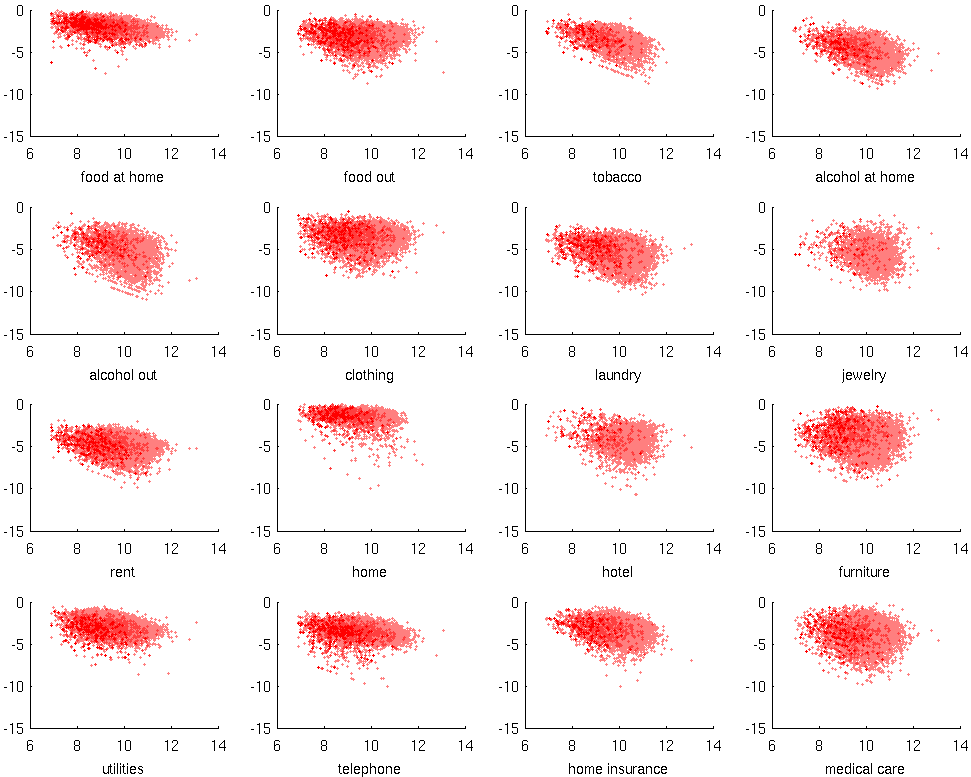
\includegraphics[scale=1]{pics/shares_cropped.pdf}
	\end{center}
	\label{fig:shr}
	\caption{Log Expenditure Shares by Log Expenditure for select goods}
\end{figure}
\begin{figure}
	\begin{center}
		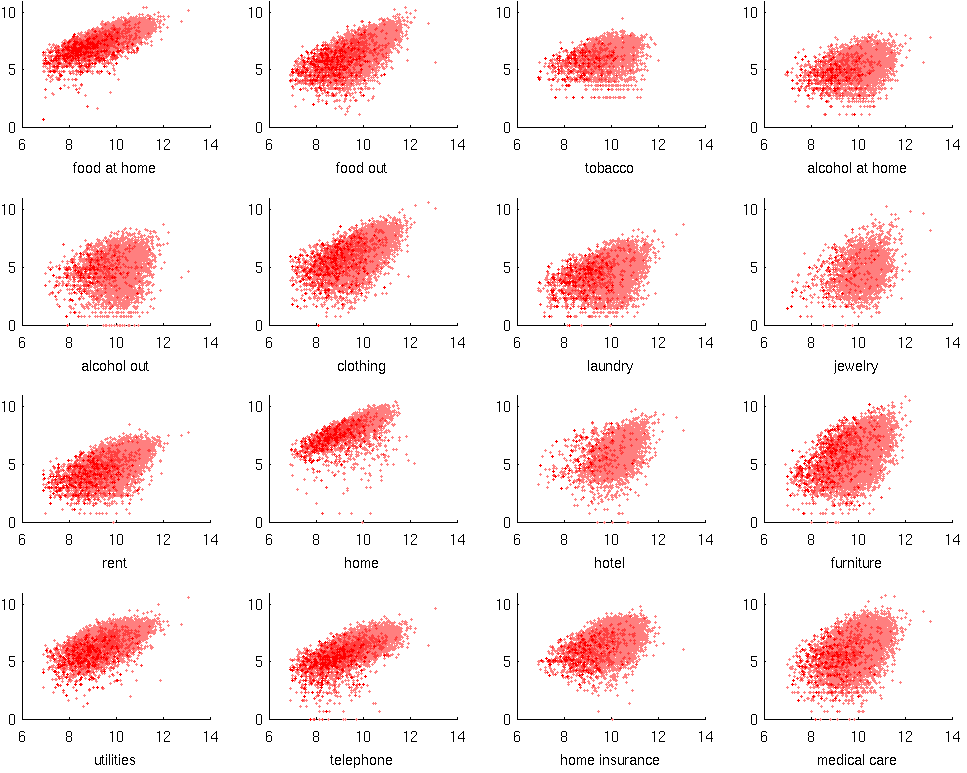
\includegraphics[scale=1]{pics/levels_cropped.pdf}
	\end{center}
	\label{fig:lev}
	\caption{Log Category Expenditure by Log Expenditure for select goods}
\end{figure}
\begin{figure}
	\begin{center}
		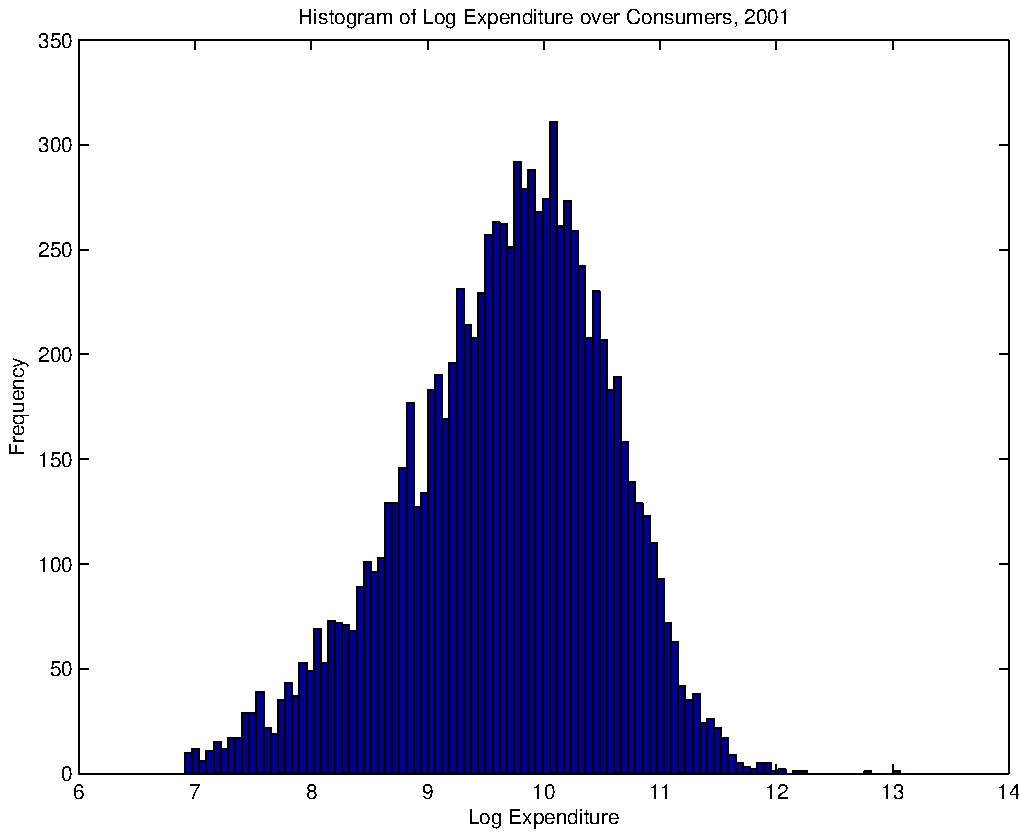
\includegraphics[scale=.8]{pics/exphist_cropped.pdf}
	\end{center}
	\label{fig:exphist}
	\caption{Histogram of  Log Expenditure}
\end{figure}
\subsection{Price Data}
I have a time-series of relative price data from the Bureau of Labor services.
Most of the NBER household consumption categories were easy to match with the definitions used by the BLS.   
Since prices are normalized to one in 1983, the units of each good which enter into the utility function are whatever one dollar could buy in 1983.
The following page is a table showing the price category names I used compared with the NBER consumption categories:

\begin{sideways}
\begin{tabular}{|l|l|l|}
\hline
VinCat Abrev & Vindex Category & PriceCatName\\ 
\hline
Brb & barbershops, beauty parlors, hair dresser, health clubs, etc. & Personal Care Services\\ 
\hline
Clo & clothing and shoes, not including underwear, undergarments and nightwear & Apparel\\ 
\hline
Cig & tobacco products like cigarettes, cigars, and pipe tobacco & Tobacco and Smoking Products\\ 
\hline
Jwl & jewelry and watches & Jewelry and watches\\ 
\hline
Car & the purchase of new and used motor vehicles such as cars, trucks, and vans & New and used motor vehicles\\ 
\hline
FdO & dining out at restaurants, drive-thrus, etc, exl. Alcohol incl. Food at school & Food away from home\\ 
\hline
Ot1 & computers, games, TVs, video, audio, musical and sports equipment, tapes, CDs. & Televisions\\ 
\hline
FdH & food and nonalcoholic beverages at grocery, specialty and convenience stores. & Food at home\\ 
\hline
Edu & education, from nursery to college, like tuition and other school expenses. & Tuition, other school fees, and childcare\\ 
\hline
Cel & mobile phone services. & Wireless Telephone Services\\ 
\hline
AlO & alcoholic beverages at restaurants, bars, cafeterias, cafes, etc. & Alcoholic Beverages away from home\\ 
\hline
AlH & alcoholic beverages for home use. & Alcoholic Beverages at home\\ 
\hline
Fur & home furnishings and household items, like furniture, appliances, tools, linen. & Furniture and bedding\\ 
\hline
Ot2 & cable TV, pets and veterinarians, sports, country clubs, movies, and concerts. & Cable and satellite television\\ 
\hline
Bks & books incl. School books, newspapers and magazines, toys, games, and hobbies. & Recreational reading materials\\ 
\hline
Cmn & vehicle maintenance, mechanical and electrical repair and replacement. & Motor vehicle maintainance\\ 
\hline
Hom & rent, or mortgage, or purchase, of housing & Housing\\ 
\hline
Htl & lodging away from home on trips, and housing for someone away at school. & other lodging away from home\\ 
\hline
Bus & public transportation, both local and long distance, like busses and trains. & Public transportation\\ 
\hline
Air & airline fares for out-of-town trips. & Airline Fare\\ 
\hline
Gas & gasoline and diesel fuel for motor vehicles. & Motor Fuel\\ 
\hline
Tel & home telephone services, not including mobile phones. & Telephone Services\\ 
\hline
Cha & contributions to churches or other religious organizations, and other charities. & Missing\\ 
\hline
Lry & laundry and dry cleaning. & Laundry equipment\\ 
\hline
Utl & home utilities such as electricity, gas, and water, garbage collection. & Fuel and Utilities\\ 
\hline
Med & medical care, incl. Health insurance, drugs, dentists, doctors, hospitals, etc. & Medical care\\ 
\hline
Fee & legal fees, accounting fees, and occupational expenses like tools and licenses. & Professional services\\ 
\hline
Cin & vehicle insurance, like insurance for cars, trucks, and vans. & Motor vehicle insurance\\ 
\hline
Hin & homeowners insurance, fire insurance, and property insurance. & Tenants' and household insurance\\ 
\hline
Lin & life insurance, endowment, annuities, and other death-benefits insurance. & Health insurance\\ 
\hline
\end{tabular}
\end{sideways}

\section{Estimation}
\subsection{Specializing to Cobb-Douglas}
Let the fundamental utility function be Cobb-Douglas:
\[u(C,\gamma) = \sum_{i=1}^{\|I\|} \gamma_i \ln(c_i)\]

Note that there is no uncertainty in the consumer's problem.
The model can be written as a generalization of the Heffetz model to many goods and preference heterogeneity.\footnote{ In the Heffetz version, there are only two goods, one visible and the other invisible to society. In my version, there is one visible good for each observation type, and all the other goods are invisible.}
Let $v\in I$ be the observation type.
Suppose that $c_v^*$ is the equilibrium consumption of the visible good.
Then the consumptions of the other goods must satisfy:
\[ U(C^*,\gamma,v|c_v^*)=\underset{\{c_i\}_{i\neq v}}{\max} \ U(C,\gamma,v|c_v^*) :  \sum_{i \neq v} r_i c_i \le W-r_v c_v^*\]
The demand for good $i\neq v$ as:
\[ c_i^* = \frac{\gamma_i}{r_i}\left(\sum_{j\neq v} \gamma_j\right)^{-1}\left(W-r_v c_v^* \right)\]
Plugging these demands into the equilibrium utility function we get:
\begin{align}
	U(C^*,\gamma,v) &= (1-\alpha)\sum_{i\neq v} \gamma_i \ln\left(\frac{\gamma_i}{r_i}\left(\sum_{j\neq v} \gamma_j\right)^{-1}\left(W-r_v c_v^* \right)\right) + h(c_v^*) \nonumber \\ 
	&= (1-\alpha) \ln\left(\prod_{j\neq v} \left(\frac{\gamma_j}{r_j}\right)^{\gamma_j}\left(\sum_{j\neq v} \gamma_j\right)^{-\sum_{j\neq v} \gamma_j}\left(W-r_v c_v^* \right)^{\sum_{j\neq v} \gamma_j}\right) + h(c_v^*) \nonumber \\ 
	\label{invop}
	&= (1-\alpha) \hat{\gamma} \ln \left(W-r_v c_v^*\right) + h(c_v^*) + (1-\alpha) \zeta(\gamma) 
\end{align}
Here $h(c_v^*)$ is the part of the utility function which does not depend upon any of the invisible goods, and:
\begin{align*}
	\hat{\gamma} &= \sum_{j\neq v} \gamma_j\\
	\zeta(\gamma) & = \ln\left(\prod_{j\neq v} \left(\frac{\gamma_j}{r_j}\right)^{\gamma_j}\left(\sum_{j\neq v} \gamma_j\right)^{-\sum_{j\neq v} \gamma_j}\right) 
\end{align*}
Note here that the budget constraint is satistfied for any choice of $c_v^* \in [0,W/r_v]$.
Society knows that given wealth and the consumption of the visible good, it is optimal to split consumption among the invisible goods as derived above.  Thus using \eqref{invop}, we can rewrite the total utility function as: 
\begin{equation}
	\label{ufun}
	U(C,\gamma,v) = (1-\alpha) \left(\hat{\gamma} \ln \left(W-r_v c_v\right) + \gamma_v \ln \left(c_v \right)\right) + \alpha \left(\gamma_v \ln \left(g(c_v)\right) + \gamma_v \ln \left(c_v\right) \right) + \zeta(\gamma)
	 \end{equation}
Here $g(c_v)$ is society's guess about $W-r_v c_v$ based on $c_v$. 
In particular, note that society's belief over a consumer's utility is described by a single-dimensional function.

The first order conditions for an interior solution to the consumer's problem can be written:
\begin{equation}
	\label{foc}
g'(c_v) = \frac{1}{\alpha}\left( \left( 1-\alpha\right) r_v - \frac{\gamma_v}{\hat{\gamma}}\frac{g(c_v)}{c_v }\right)
\end{equation}

Now we can directly follow Heffetz and solve this differential equation:
\begin{equation}
	\label{difsol}
	g(c_v) = \frac{\hat{\gamma}\left(1-\alpha\right)}{\gamma_v +\alpha \hat{\gamma}} r_v c_v + K c_v^{-\frac{\gamma_v}{\alpha \hat{\gamma}}}
\end{equation}
To solve for the constant $K$, note that the lowest possible wealth type $\underbar{W}$ has no reason to signal in a separating equilibrium.
In particular, his consumption will not be distorted, so that his demand $\underbar{c}$ for $c_v$ will be given by:
\begin{equation}
	\label{lowc}
	\underbar{c} = \frac{\gamma_v}{r_v}\left(\sum_{j} \gamma_j\right)^{-1}\underbar{W} 
\end{equation}
Since in equilibrium $g(\underbar{c}) = \underbar{W} - r_v \underbar{c}$, we can plug into \eqref{difsol} and solve for $K$:
\[
K = \frac{\underbar{W}- \frac{\gamma_v + \hat{\gamma}}{\gamma_v + \alpha \hat{\gamma}}r_v \underbar{c}}{\underbar{c}^{-\frac{\gamma_v}{\alpha \hat{\gamma}}}}
\]
We can think of $g$ as a function of $c_v$ and $\underbar{W}$. 
Then $g$ is jointly homothetic.  
\footnote{
Below I show that $g$ is jointly homothetic of degree one in $\underbar{W}$ and $c_v$.  First, it is immediate from \eqref{lowc} that $\underbar{c}$ scales linearly with $\underbar{W}$.
Now $K$ scales non-linearly with $\underbar{W}$:
\begin{align*}
	K(s\underbar{W}) &= \frac{s\underbar{W}- \frac{\gamma_v + \hat{\gamma}}{\gamma_v + \alpha \hat{\gamma}}r_v s \underbar{c}}{(s\underbar{c})^{-\frac{\gamma_v}{\alpha \hat{\gamma}}}} \\
	&= s^{1 + \frac{\gamma_v}{\alpha \hat{\gamma}}}K(\underbar{W})
\end{align*}
The way $K$ scales, however, is just right to make $g$ scale linearly in $c_v$:
\begin{align*}
	g(s c_v,\underbar{W}) &= \frac{\hat{\gamma}\left(1-\alpha\right)}{\gamma_v +\alpha \hat{\gamma}} r_v s c_v + s^{1+\frac{\gamma_v}{\alpha \hat{\gamma}}} K(\underbar{w}) (s c_v)^{-\frac{\gamma_v}{\alpha \hat{\gamma}}} \\
	&= \frac{\hat{\gamma}\left(1-\alpha\right)}{\gamma_v +\alpha \hat{\gamma}} r_v s c_v + s K(\underbar{w}) c_v^{-\frac{\gamma_v}{\alpha \hat{\gamma}}} \\
	&= s g(c_v,\underbar{W})
\end{align*}
}
This means that, given prices, a scaling of social wealth just scales consumption choices.
\footnote{
In this footnote, I show that if $c^*$ is an interior maximizer of \eqref{ufun} for an individual of wealth $W$, then $s c^*$ is a solution to the  problem of an individual of wealth $s W$, as long as we also scale $\underbar{W}$ up by $s$ as well.
If $c^*$ is an interior maximizer, then it solves the first order conditions of \eqref{ufun}:
\[
\frac{(1-\alpha)r_v \hat{\gamma}}{W-r_v c^*} = \frac{\alpha \gamma_v g'(c^*)}{g(c^*)} + \frac{\gamma_v}{c^*}
\]
Now divide both sides of the equation by $s$, and using the fact that $g$ is homothetic of degree one and $g'$ is homothetic of degree zero, we get:
\[
\frac{(1-\alpha)r_v \hat{\gamma}}{s W-r_v s c^*} = \frac{\alpha \gamma_v g'(s c^*)}{g(s c^*)} + \frac{\gamma_v}{s c^*}
\]
Thus, $s c^*$ solves the scaled problem.
}
\subsection{Derivation of Estimation Equations}
The strategy in this section is to use maximum likelihood to estimate the parameters of the model.  
While there is no uncertainty in the model for consumers, their are two parameter sets that are unobserved by the econometrician.
The first is a latent variable--the observation type.
The second is preference heterogeneity.
As is standard in this type of problem, I proceed with the EM algorithm.
In the first step, I randomly assign each household an observation type.
Then I get parameters by maximizing the likelihood with respect to preference heterogeneity.
Next I use the model parameters to assign the observation types with the highest likelihood.
Using these observation types, I get a new set of parameters using maximum likelihood over the preference heterogeneity.
This process is repeated until there is no reassignment of observation type.

The first order of business is to derive the likelihood function.
As a reminder, the utility function now looks like this:
\begin{equation}
	\label{totuti}
U(C,\gamma,v) = (1-\alpha) \sum_{j=1}^{29}\gamma_j \ln(c_j )  + \alpha \left(\gamma_v \ln(c_v)+ \hat{\gamma}\ln(g(c_v,v,\gamma))  + \zeta \right)
\end{equation}

%I assume that the preference shocks $\gamma$ are distributed exponential with rate parameter $\lambda_i$. 
%The exponential distribution is convenient because there are many zeros in the data, which imply a $\gamma$ of zero in the model.
%The exponential distribution has positive density at zero.
%I considered choosing the $\Gamma$ distribution, but this adds another parameter to estimate for each good, and the shape of $\gamma$ is not too different from that of the exponential distribution for the range of parameters which give positive density at zero.
I assume that the preference parameters are distributed log normal with a mass point at zero.
This assumption seems reasonable given the raw data.
First of all, Table \ref{tab:sharetab} shows that there is a lot of mass at zero.
\begin{table}
	\begin{center}
\begin{tabular}{|l|c|}
	\hline
\textbf{Category} & \textbf{Zero Expenditure} \\
	\hline
Clo (clothing) & 0.11 \\ 
	\hline
Cig (cigarettes) & 0.60 \\ 
	\hline
Car (cars) & 0.47 \\ 
	\hline
Fur (furniture) & 0.26 \\ 
	\hline
Ot1 (recreation 1) & 0.16 \\ 
	\hline
Jwl (jewelry) & 0.64 \\ 
	\hline
FdO (food out) & 0.10 \\ 
	\hline
AlH (alcohol home) & 0.49 \\ 
	\hline
AlO (alcohol out) & 0.51 \\ 
	\hline
Ot2 (recreation 2) & 0.10 \\ 
	\hline
Brb (barbers etc) & 0.17 \\ 
	\hline
Bks (books etc) & 0.48 \\ 
	\hline
Edu (education) & 0.70 \\ 
	\hline
Hom (rent/home) & 0.57 \\ 
	\hline
FdH (food home) & 0.02 \\ 
	\hline
Htl (hotels etc) & 0.62 \\ 
	\hline
Air (air travel) & 0.67 \\ 
	\hline
Bus (public trans.) & 0.73 \\ 
	\hline
CMn (car repair) & 0.24 \\ 
	\hline
Cha (charities) & 0.58 \\ 
	\hline
Gas (gasoline) & 0.11 \\ 
	\hline
Lry (laundry) & 0.33 \\ 
	\hline
Med (health care) & 0.25 \\ 
	\hline
Tel (home phone) & 0.06 \\ 
	\hline
Utl (home utilities) & 0.12 \\ 
	\hline
Fee (legal fees) & 0.36 \\ 
	\hline
CIn (car insur.) & 0.35 \\ 
	\hline
LIn (life insur.) & 0.54 \\ 
	\hline
HIn (home insur.) & 0.41 \\ 
	\hline
\end{tabular}
\end{center}
\label{tab:sharetab}
\caption{Fraction with zero shares in household expenditures by category.}
\vspace{-2in}
\end{table}
The highest zero consumption rate is public transportation at 73.44\%.  
Given the Cobb-Douglas structure of utility, the only way to get exactly zero consumption is with a utility parameter of zero.
The justification for the log-normal assumption is due to Figure .
\begin{figure}
	\begin{center}
		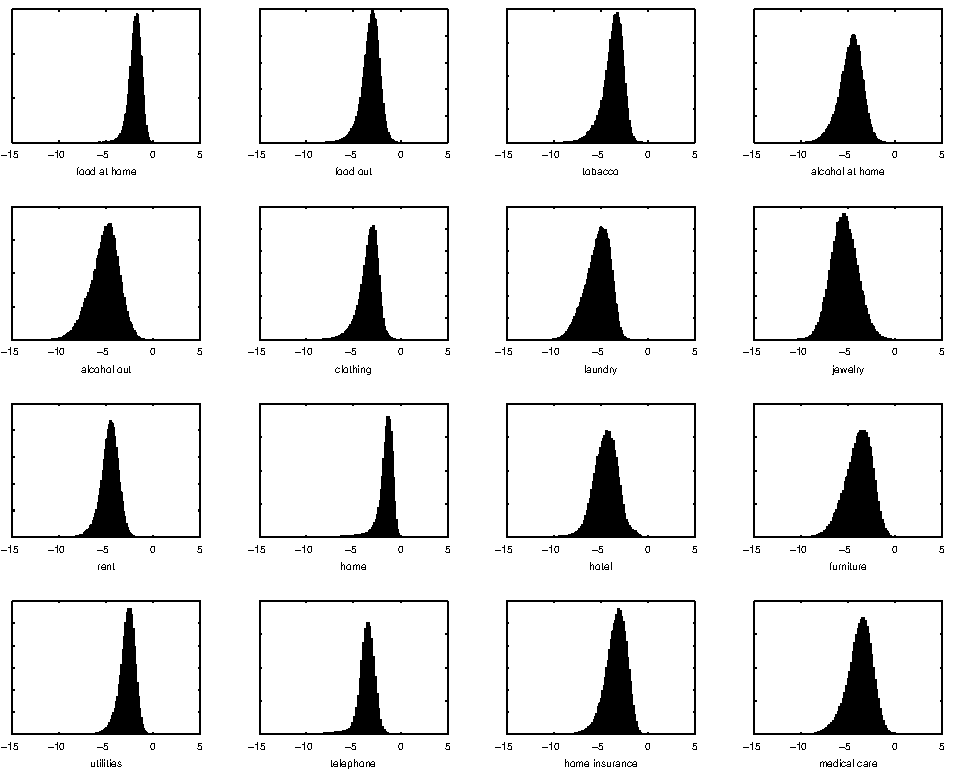
\includegraphics[scale=1]{pics/shrplot_cropped.pdf}
	\end{center}
	\caption{Log non-zero consumption share histograms by category.}
	\label{fig:shrplot}
\end{figure}
Figure  shows histograms of the logs of non-zero expenditures for the first 16 consumption categories.  
The histograms are all reasonably close to normal probability distribution functions.
If there was no signaling, Cobb-Douglas utility would imply that consumption shares are directly proportional to utility parameters.
The signaling model retains a Cobb-Douglas flavor, as shares of non-observable goods are still proportional to utility parameters.
Choosing a log-normal distribution with a zero mass point gives me enough flexibility to capture the general shape of the data.

Consider a household of wealth type $W$ and with consumption vector $C$.  
Suppose that the household is observation type $v$.
Then the consumptions of goods $j\neq v$ are given by:
\begin{align}
	\label{eq:sgd}
	r_jc_j &= \frac{\gamma_j}{\sum_{i\neq v}\gamma_i}  \left(W-  r_v c_v\right)\\
	\label{eq:sgdsol}
	\gamma_j &= \frac{r_j c_j}{\left(W- r_v c_v\right)} \sum_{i\neq v}\gamma_i  
\end{align}

We can solve for the 28 $\gamma$'s up to a scaling factor $\sum_{i\neq v}\gamma_i$.
I normalize the parameter $\gamma_1$ on consumption of food at home to one. 
\footnote{It is important to choose a good which always has positive consumption, since this strategy will not work if consumption of the normalized good is zero.  
Fortunately, food at home is consumed in all but (x) of the households.}
If food at home is not the observation type, and in what follows I assume it is not, then the solution for $j \neq v$ is:
\footnote{In a previous version of the estimation, I allowed for food at home to be an observation type.
It is not difficult to do so.
The only drawback is that the numerical optimization comes first (and solves for $\sum_{j \neq 1} \gamma_j$ rather than $\gamma_1$ which is normalized to unity.  
Putting the numerical optimization in the first step potentially adds some error into the coefficients in the second step, and I found that the estimation routine became very touchy with regard to starting values.
In any case, for now I assume that food at home is not the observation type.
This assumption may not be too serious since food at home is a relatively invisible consumption category.
}
\begin{equation}
	\label{eq:gamsol}
	\gamma_j = \frac{r_j c_j}{r_1 c_1}
\end{equation}
Using the first order conditions to the consumer's problem \eqref{foc} and given the results of \eqref{eq:gamsol}, for each household I numerically solve for  $\gamma_v$.
%We are still missing $\gamma_v$ from the good which society observes.
%$\gamma_v$ can be approximated by using the implicit function theorem and a Taylor expansion around the optimal consumption of the visable good for some predetermined value $\hat{\gamma}_v$, for example the mean of the distribution in the last iteration.  Appreviating the $g(c,v,\gamma)$ function with $g(c_v)$ we have:
%\begin{equation}
%	\frac{\partial \gamma_v}{\partial c_v(\hat{\gamma}_v)}|c_v(\hat{\gamma}_v) =\frac{\gamma_v}{c_v(\hat{\gamma}_v)}-\alpha \frac{c_v(\hat{\gamma}_v) g''(c_v(\hat{\gamma}_v))\sum_{j\neq v} \gamma_j }{g(c_v(\hat{\gamma}_v))}+\alpha \frac{c_v(\hat{\gamma}_v) (g'(c_v(\hat{\gamma}_v)))^2 \sum_{j\neq v}\gamma_j}{(g(c_v(\hat{\gamma}_v)))^2} + \frac{r_v^2 c_v(\hat{\gamma}_v)}{(W-r_v c_v(\hat{\gamma}_v))^2}
%\end{equation}
%
%The approximation is then:
%\begin{equation}
%	\gamma_v \approx \hat{\gamma}_v + \left(\frac{\partial \gamma_v}{\partial c_v(\hat{\gamma}_v)}|c_v(\hat{\gamma}_v)\right) \left(c_v - c_v(\hat{\gamma})\right)
%\end{equation}
%
%If the observation type \emph{is} food at home, then the situation changes a little bit.  
%The first step is to use a similar approximation to solve for $\sum_{j\neq 1} \gamma_j$, around some value $\hat{\gamma}^*$:
%\begin{equation}
%	\frac{\partial \hat{\gamma}}{\partial c_v(\hat{\gamma})}|c_v(\hat{\gamma}^*) = \frac{g(c_v(\hat{\gamma}^*))}{\alpha g'(c_v(\hat{\gamma}^*))}\left(\frac{1}{c_v(\hat{\gamma}^*)} + \frac{r_v^2}{W-r_v c_v(\hat{\gamma}^*))}\right) + \hat{\gamma}^* \left(\frac{g'(c_v(\hat{\gamma}^*))}{g(c_v(\hat{\gamma}^*))} - \frac{g''(c_v(\hat{\gamma}^*))}{g'(c_v(\hat{\gamma}^*))}\right)
%\end{equation}
%And the approximation, as above:
%\begin{equation}
%	\hat{\gamma} \approx \hat{\gamma}^* + \left(\frac{\partial \hat{\gamma}}{\partial c_v(\hat{\gamma})}|c_v(\hat{\gamma}^*)\right) \left(c_v - c_v(\hat{\gamma}^*)\right)
%\end{equation}
%Once we have an approximation of $\sum_{j\neq 1} \gamma_j$, we can easily solve the simultaneous equations \eqref{eq:sgdsol}.
It should be noted that to get the $g$ function in the first order condition \eqref{foc}, I need to estimate the lowest social wealth level. 
At first blush, it appears that using the minimum wealth level in my data set would be a good estimator for this wealth level.
Presumably due to measurement error, however, the data set contains a few unbelievably low values--the lowest (positive) value is something on the order of six dollars of annual expenditure.
In practice, I assume the lowest possible wealth level is one thousand dollars, and drop any households with lower expenditure.
Out of my 160,617 household observations, 4722 are dropped because they are less than 1000 dollars, 1079 further observations are dropped due to negative consumption reports, and finally 800 further observations are dropped due to zero expenditures on food at home.
This leaves me with a total of 154,016 usable observations.
For completeness, I include the likelihood function for a single household below.  $\gamma_j$ is a function of observed consumption $C$ and observation type $v$, but to simplify notation I just write $\gamma_j$:
\begin{equation}
	\label{lik1}
	l(C|v,\mu,\sigma) = \sum_{j} \left(\mathbf{1}_{\{\gamma_j = 0\}}\ln\left(pr(\gamma_j=0)\right)) + \mathbf{1}_{\{\gamma_j \neq 0\}} \left(\ln\left(1-pr(\gamma_j = 0)\right)+\ln \phi(\gamma_j|\mu_j,\sigma_j)\right)\right)
\end{equation}
Here $\phi$ is the log-normal probability density function.

Once we have solved for the distribution parameters, we can calculate a likelihood for each observation type possibility.
Up to this point, I have not introduced the Heffetz vindex into the estimation. The vindex enters in the next step (the E step in the EM algorithm).
Given a set of parameters, we need to choose the most likely observation type for each household.
This calculation for each household is as follows:
\begin{equation}
	\max_{i\in I} \ln (v_i) + l(C|i,\mu,\sigma)
\end{equation}
The $v_i$ here is the vindex probability, or the probability of social group judging well-being based on a particular good category.
In practice I have different visibility indexes for four groups of households: blacks under 40, blacks over 40, non-blacks under 40, and non-blacks over 40.
The visibility probabilities are taken directly from Heffetz and normalized so that they sum to one.
\footnote{A household is identified by the self-identified characteristics of whoever answered the consumption survey. 
In a previous version of this project, I needed to calculate equilibrium consumptions for each type.  This led me to keep the type nmber small.  In the current version, the fineness of the type does not affect the speed of estimation.  One of the next things on the plate, in terms of this project, is including very fine types--as fine as allowed by the Heffetz survey.}

There are 28 $\mu$'s, 28 $\sigma$'s, 28 zero mass point probabilities, and $\alpha$ to be estimated--a total of 85 parameters.   
In my useable dataset, I have 154,016 households which is 1,800 household observations per parameter.
However, to save computation time, I am currently using only 10,000 randomly chosen household observations, or a little over 100 observations per parameter.
Since the preference heterogeneity is assumed to be independent, given observation types and an $\alpha$ I can use the (log) sample mean and variance to recover the likelihood maximizing $\mu$ and $\sigma$'s.
Thus the maximization step above is really only over the single dimensional $\alpha$ parameter.
%\section{Discussion of Estimation}
%The overhead of passing information back and forth between cores with such quick tasks makes is quicker to just use a standard serial process.
%The typical way to solve this problem is to group the small tasks into larger tasks to be passed to individual cores.  
%In any case, this is probably the next thing I will implement in the code.
%
%With 10,000 observations, it takes about two seconds to evaluate the likelihood function once.
%Since the solver I am using (knitro) needs to approximate the jacobian at each iteration, one iteration of the likelihood solver takes about two minutes.
%The second step in which the most likely observation types are chosen takes a bit longer to run one iteration, but usually only needs to run onc or two iterations before the EM algorithm converges stops.
%
%One issue is the appearance of NaNs and infs in the likelihood estimation. 
%This happens occasionally, and rather than kill the loop I currently just penalize the likelihood.
%I do this by adding a log likelihood value about ten times worse than the minimum of likelihood values appearing in a typical run.
%The infs appear when the likelihood is very low, so that MATLAB approximates with zero.
%I haven't been able to diagnose the occassional NaN yet.
\section{Results}
Table \ref{tab:parest} below presents estimation results.  
\begin{table}
	\begin{center}
		\begin{tabular}{|l|c c |c c |c c|}
			\hline
			Good Cat & $\mu$ & std err      & $\sigma$ & std err       & $pr(\gamma_j =  0)$ & std err\\
			\hline
			FdO & -1.2106 &  (0.0002) &  1.1823 & (0.0005) &   0.0836 & (0.0038)\\ 
			\hline
			Cig & -6.1907 &  (0.0022) & 11.4001 & (0.0512) &   0.8274 & (0.0054)\\ 
			\hline
			AlH & -2.7418 &  (0.0002) &  1.2418 & (0.0006) &   0.4760 & (0.0070)\\ 
			\hline
			AlO & -3.0832 &  (0.0003) &  1.6011 & (0.0010) &   0.5032 & (0.0070)\\ 
			\hline
			Clo & -1.4358 &  (0.0002) &  1.1580 & (0.0005) &   0.0938 & (0.0040)\\ 
			\hline
			Lry & -3.3559 &  (0.0002) &  1.3826 & (0.0007) &   0.3102 & (0.0065)\\ 
			\hline
			Jwl & -5.3608 &  (0.0015) &  8.1810 & (0.0228) &   0.6604 & (0.0067)\\ 
			\hline
			Brb & -2.6958 &  (0.0002) &  1.0096 & (0.0004) &   0.1530 & (0.0050)\\ 
			\hline
			Hom &  0.3824 &  (0.0002) &  0.8689 & (0.0004) &   0.7046 & (0.0065)\\ 
			\hline
			Htl & -2.4135 &  (0.0002) &  1.3596 & (0.0007) &   0.6360 & (0.0068)\\ 
			\hline
			Fur & -1.9858 &  (0.0002) &  1.4964 & (0.0008) &   0.2570 & (0.0061)\\ 
			\hline
			Utl & -0.8731 &  (0.0001) &  0.7561 & (0.0002) &   0.0960 & (0.0041)\\ 
			\hline
			Tel & -1.6308 &  (0.0001) &  0.9058 & (0.0003) &   0.0360 & (0.0025)\\ 
			\hline
			HIn & -1.5132 &  (0.0002) &  1.1389 & (0.0005) &   0.4102 & (0.0069)\\ 
			\hline
			Med & -1.8537 &  (0.0002) &  1.3468 & (0.0007) &   0.2514 & (0.0061)\\ 
			\hline
			Fee & -2.9173 &  (0.0002) &  1.3449 & (0.0007) &   0.3530 & (0.0067)\\ 
			\hline
			LIn & -2.2290 &  (0.0002) &  1.2182 & (0.0006) &   0.5192 & (0.0070)\\ 
			\hline
			Car & -2.3967 &  (0.0003) &  1.8427 & (0.0013) &   0.5890 & (0.0069)\\ 
			\hline
			CMn & -2.2251 &  (0.0003) &  1.5484 & (0.0009) &   0.2236 & (0.0058)\\ 
			\hline
			Gas & -1.0737 &  (0.0001) &  0.8481 & (0.0003) &   0.0956 & (0.0040)\\ 
			\hline
			CIn & -1.4963 &  (0.0001) &  0.8789 & (0.0003) &   0.3360 & (0.0066)\\ 
			\hline
			Bus & -6.1303 &  (0.0014) &  8.6399 & (0.0211) &   0.7626 & (0.0060)\\ 
			\hline
			Air & -2.2693 &  (0.0003) &  1.6096 & (0.0010) &   0.6914 & (0.0065)\\ 
			\hline
			Bks & -3.4553 &  (0.0002) &  1.4929 & (0.0008) &   0.4718 & (0.0070)\\ 
			\hline
			Ot1 & -2.7484 &  (0.0002) &  1.1775 & (0.0005) &   0.1316 & (0.0047)\\ 
			\hline
			Ot2 & -1.3021 &  (0.0002) &  1.2837 & (0.0006) &   0.0828 & (0.0038)\\ 
			\hline
			Edu & -5.8550 &  (0.0019) & 10.3474 & (0.0383) &   0.8262 & (0.0054)\\ 
			\hline
			Cha & -2.3950 &  (0.0003) &  1.5843 & (0.0010) &   0.5950 & (0.0069)\\ 
			\hline
		        \hline	
			$\alpha$ & 0.1459 & (0.0071) & & & & \\
			\hline
			\hline
		\end{tabular}
	\end{center}
	\caption{Parameter Estimates}
	\label{tab:parest}
\end{table}
The main parameter of interest, the weight of conspicuous consumption in utility, is a reasonable 0.1459.  
Qualitatively, cigarettes, jewelry, and education have particularly low $\mu$'s and high $\sigma$'s. 
This says that most people care very little about these goods, but some people spend care very deeply for them.
The reason the estimates come out this way is that most households spend very little on jewelry, cigarettes, and education, but some households spend large somes in these categories. 

Figure and figure are scatter plots of simulated data, made in the same way as the scatter plots of the actual data in figures \ref{fig:shr} and \ref{fig:lev}. 
\begin{figure}
	\begin{center}
		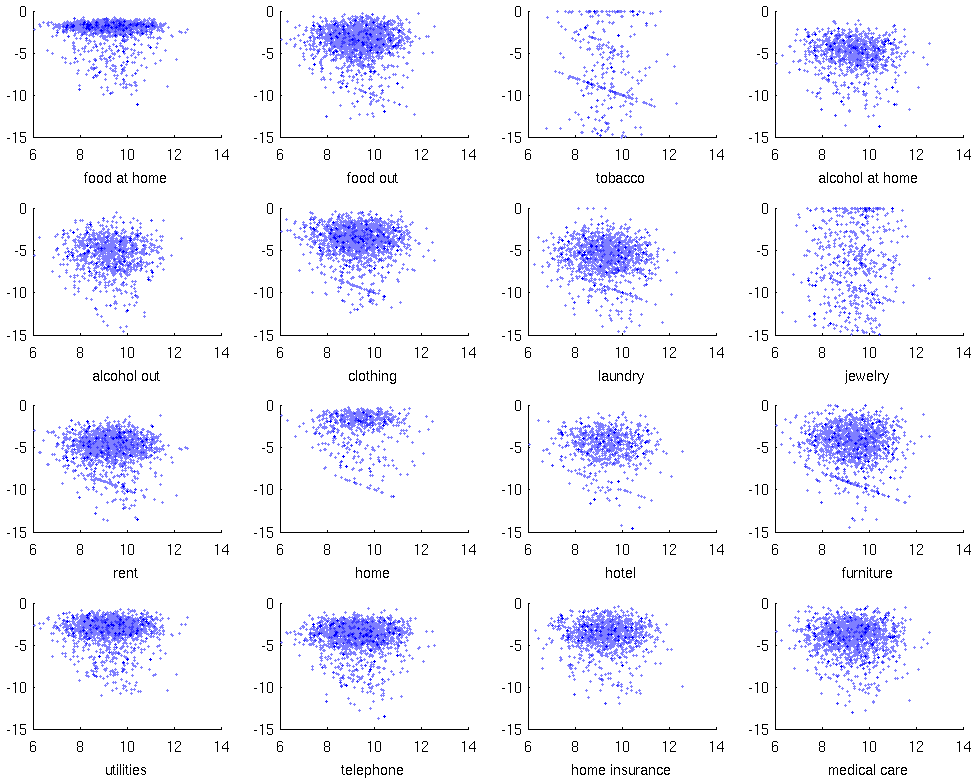
\includegraphics[scale=1]{pics/shares_fake_cropped.pdf}
	\end{center}
	\caption{Simulated expenditure share plots by category.}
	\label{fig:shares_fake}
\end{figure}
\begin{figure}
	\begin{center}
		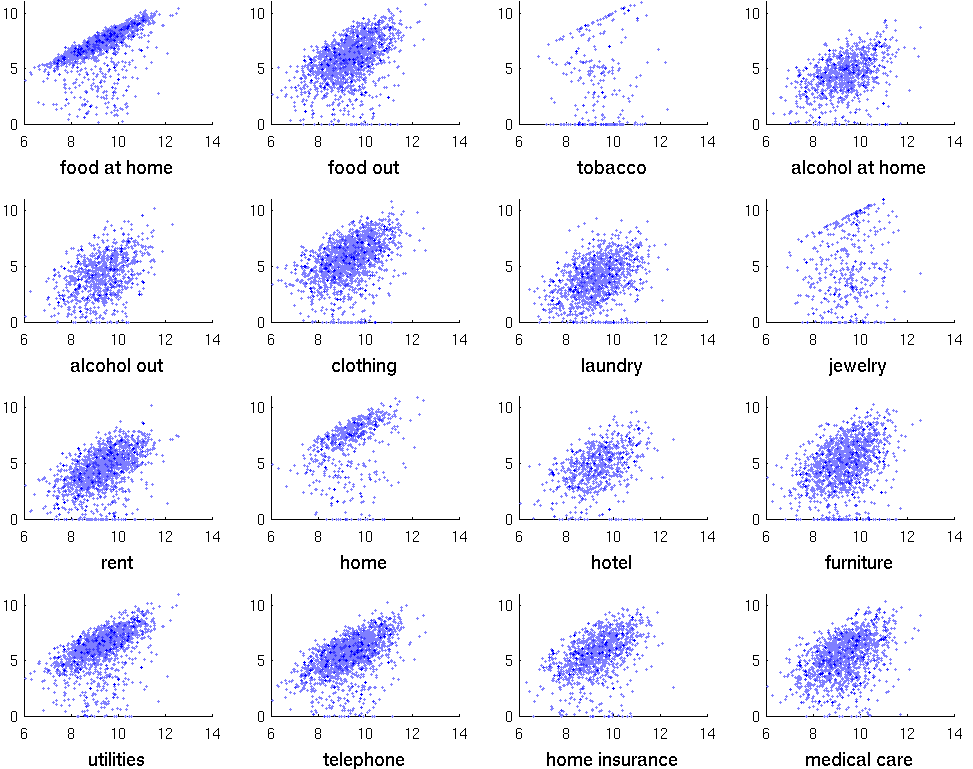
\includegraphics[scale=1]{pics/levels_fake_cropped.pdf}
	\end{center}
	\caption{Simulated expenditure level plots by category.}
	\label{fig:levels_fake}
\end{figure}
The simulated data only have 5000 observations compared with the full dataset's upwards of 150,000 observations. 
Besides the sparcity, however, the simulated data looks quite similar to the actual data.

The estimation does less well on observation types.
Ideally the observation type distribution (for a particular demographic) should be the same as the vindex probability distribution from the Heffetz survey.
The estimated observation type densities, however, have only a $0.3778$ correlation with the vindex probabilities.
Figure \ref{fig:vinmatch} is a scatter plot of the vindex probabilities and the estimated observation type densities.
\begin{figure}
	\begin{center}
		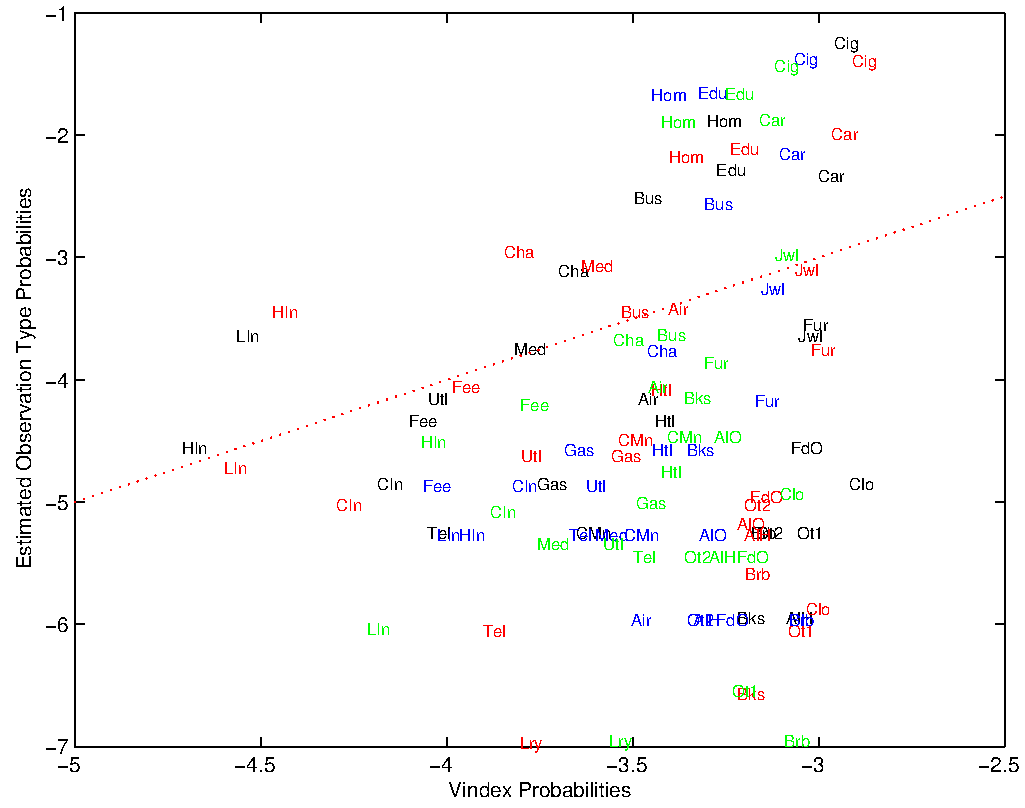
\includegraphics[scale=.8]{pics/vinmatch_cropped.pdf}
	\end{center}
	\caption{Estimated (log) observation type distribution compared to (log) Heffetz vindex.}
	\label{fig:vinmatch}
\end{figure}
Each point is labeled with the relevant good category, and the colors represent different demographic types (black or not, under or over 40).
The estimated probabilities are exagerated compared with the vindex probabilities.
I do not have good intuition about why this happens.

\subsection{Welfare experiments}
Now that we have an estimated model, we can talk about the welfare costs of signaling.
Consider a typical consumer (with the modal preference parameter for each category) of various wealth levels.  
Figure \ref{fig:uchnge} plots percentage gain in utility over expenditures (from 1000-20,000 dollars a year) for the 28  observation types.
I broke out housing because the gain was much higher than in the other observation types.
As we would  predict, the wealthier a household is, the more it has to gain from eliminating signaling.
This is because wealthier households need to distort their consumption more to signal their wealth. 
To see this, note that the poorest household gains nothing from an elimination of signaling, since the poorest household has nothing to gain from signaling anyway.

\begin{figure}
	\begin{center}
		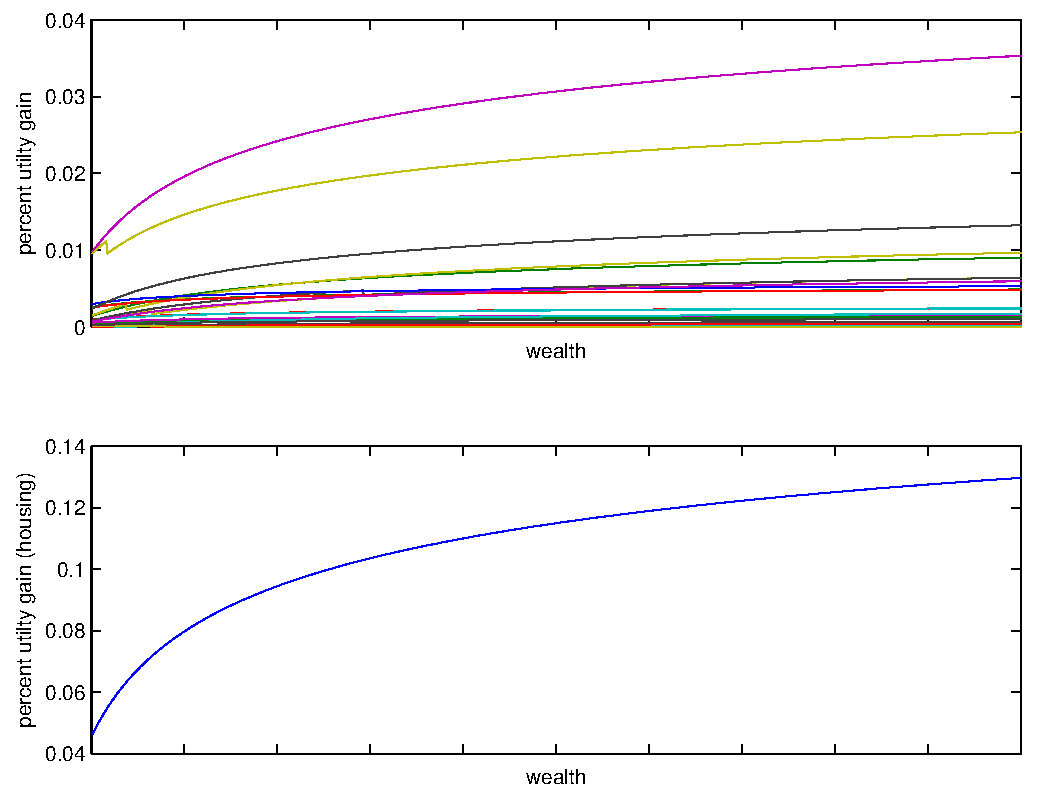
\includegraphics[scale=.8]{pics/uchnge_cropped.pdf}
	\end{center}
	\caption{Percentage welfare gain due to the elimination of signaling, by observation type}
	\label{fig:uchnge}
\end{figure}

\section{Optimal Taxes}
There is scope in this environment for welfare-increasing taxes.  
In what follows I consider an excise tax, the revenue of which is passed back to consumers in proportion to their wealth.
Here I use the homotheticity result at the end of Section 2 so that this redistribution scheme does not change budget shares.
I do not want to introduce the supply side into this model.
The operating assumption is that taxes affect neither firm pricing decisions nor worker wages.
\footnote{
A cheap and totally uninteresting way to embed this assumption in general equilibrium would be to assume that inelastically supplied effective labor is the only input into a linear production function, and that there is perfect competition between firms.
Since the prices paid to firms do not change if we impose taxes, wages do not adjust.
Production is just scaled up or down depending on the demand effect of the taxes.
}
A tax assessed on a relatively visible good has two effects.
Intuitively, people overconsume visible goods.
As a visible good increases in price, a smaller proportion of wealth is spent on the visible good.
Since taxes are completly passed back lumpsum to consumers (with a caveat), no wealth is lost.
There is just less distortion in equilibrium.

With the tax scheme I am implementing, there is also a redistributive effect.
Since the rich distort consumption the most in order to signal, the first affect mostly helps them.
However, tax revenues are passed back in proportion to wealth.
The more wealthy a consumer is, the higher the share her budget she spends on the visible good
A rich consumer pays more tax per unit wealth than she receives back from the government.
Thus the poor are also made better off by an excise tax on a visible good.  
The goal is to find a set of non-negative excise taxs that maximizes the sum of all utilities in a society.

Once we have the distribution of utility parameters, it is straightforward to numerically solve for the optimal tax.
First I simulate a thousand individuals.
Utility parameters are randomly drawn from the estimated distributions.
Wealth levels are drawn from the total expenditure distribution in the data for a single year, the year 2000.
Prices are also those from the year 2000.
Observation types are drawn from estimated distribution of a single type (non-black, under 40).
Then I use a numerical solver to search over good category specific taxes in order to maximize the unweighted sum of each individual's utility.
In an inner loop, I use the prices implied by a set of taxes to numerically solve for optimal consumption for each consumer.
Using the homotheticity result, I can just scale up each consumer's optimal consumption by the tax revenue.
\footnote{It is a little more subtle than this, since some of what is redistributed back to consumers is again collected in taxes.
Thus expenditures are actually scaled up by a geometric sum of the proportion of total expenditure which is collected as taxes. 
}
Utility is then calculated and passed back to the outer loop.

Optimal taxes are expressed as a multiple of base prices in Table \ref{tab:opttax}.
\begin{table}
	\begin{center}
		\begin{tabular}{|l|c|}
			\hline
			\textbf{Good Cat} & \textbf{Tax} \\
			\hline
			FdH &  3.7860\\
			\hline
			FdO &  1.5188\\ 
			\hline
			Cig &  8.4272\\ 
			\hline
			AlH &  2.1151\\ 
			\hline
			AlO &  0.0761\\ 
			\hline
			Clo &  1.1873\\ 
			\hline
			Lry &  0.0000\\ 
			\hline
			Jwl &  3.1023\\ 
			\hline
			Brb &  0.0000\\ 
			\hline
			Hom &  8.8748\\ 
			\hline
			Htl &  0.0733\\ 
			\hline
			Fur &  0.9623\\ 
			\hline
			Utl &  1.9966\\ 
			\hline
			Tel &  0.9322\\ 
			\hline
			HIn &  0.3863\\ 
			\hline
			Med &  0.7386\\ 
			\hline
			Fee &  0.0000\\ 
			\hline
			LIn &  0.5304\\ 
			\hline
			Car &  1.1046\\ 
			\hline
			CMn &  2.0361\\ 
			\hline
			Gas &  2.2456\\ 
			\hline
			CIn &  0.5941\\ 
			\hline
			Bus &  2.7202\\ 
			\hline
			Air &  2.2799\\ 
			\hline
			Bks &  0.0000\\ 
			\hline
			Ot1 &  0.0000\\ 
			\hline
			Ot2 &  1.5486\\ 
			\hline
			Edu &  1.2739\\ 
			\hline
			Cha &  1.3754\\ 
			\hline
		\end{tabular}
	\end{center}
	\caption{Optimal taxes as multiple of base price}
	\label{tab:opttax}
\end{table}
Optimal taxes can be quite large--in the case of cigarettes and homes, the price is raised by a factor of eight.
The reason these taxes are so high is that many people signal with home and cigarette consumption.
In fact, the estimated distribution of observation types is strongly correlated with optimal taxes.
Figure \ref{fig:tvscat} is a scatter plot of log estimated observation types and log tax adjusted prices.
\begin{figure}
	\begin{center}
		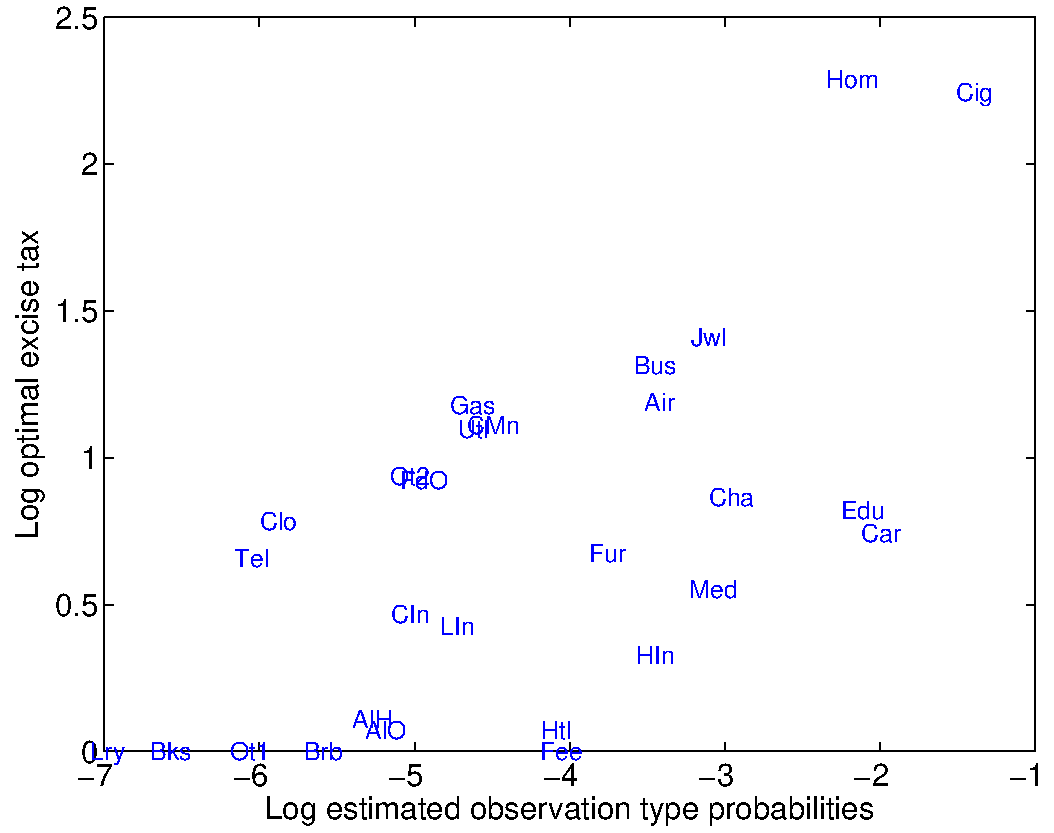
\includegraphics[scale=.8]{pics/tvscat_cropped.pdf}
	\end{center}
	\caption{Scatter plot of log estimated observation type probability and log post-tax price}
	\label{fig:tvscat}
\end{figure}
I present the simulated utility gain for each of the thousand simulated consumers in Figure \ref{fig:taxscat}.
\footnote{I trimmed four outliers for presentation.
One outlier had large utility loss, around -30\%, and the others had very large utility gains.}
\begin{figure}
	\begin{center}
		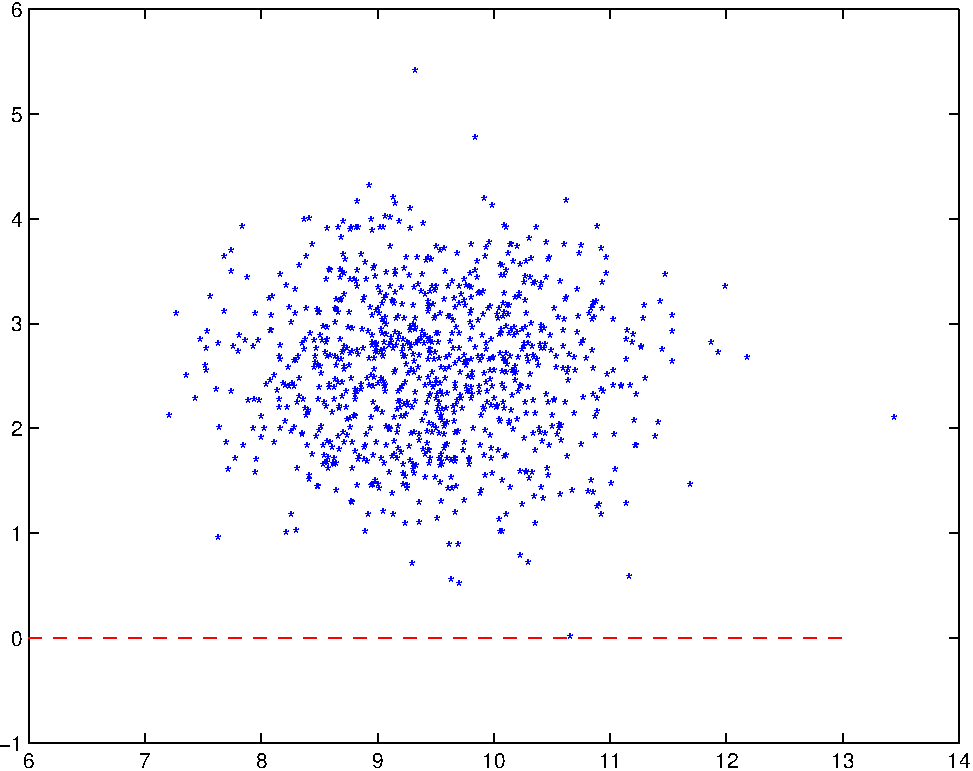
\includegraphics[scale=.8]{pics/taxscat_cropped.pdf}
	\end{center}
	\caption{Percentage utility change under optimal tax regime by log wealth}
	\label{fig:taxscat}
\end{figure}
Note that not everyone gains from the optimal tax.  
The taxes hurt people who happen to have uncommon observation types.
Since these goods become relatively cheap, these consumers must buy large amounts to signal their wealth, and thus their consumption profiles become more distorted.
However, a large majority of consumers gain from the tax regime.
The median welfare increase is 3.4\%, and the mean is 3.7\%.
\section{Conclusion}
This paper takes a conspicuous consumption model from the theory literature seriously by adding preference heterogeneity and estimating parameters from data.
The results of the estimation show that signaling may play an important role in consumption decisions.
About 14.6\% of a consumers actual well-being is due to his social group's belief about his well-being.
This fairly large number means that taxing the goods which are frequently used as signals of well-being may lead to significant welfare increases.
A simulation suggests a median welfare increase of 3.4\%.
In India, a tax on festival spending might increase the welfare of the poorest Indians.
In the United States, I suggest a large tax on Apple products.

In order to get an estimable model, I had to make a few unrealistic assumptions.
One's social group sees only consumption expenditures in one good category. 
This is clearly counterfactual.
In the real world, one's social group sees a full vector of consumption expenditures, but with some noise.
An earlier version of this paper had a model with this feature, but estimation involved numerically calculating a thirty dimensional integral for each consumer for each parameter trial.
Future research might focus on finding a tractible model to estimate without such a stark assumption about the observability of consumption.
\bibliographystyle{plainnat}
\bibliography{biglist.bib}
\end{document}
